\section{Methodology}

\begin{figure}[h]
    \centering
    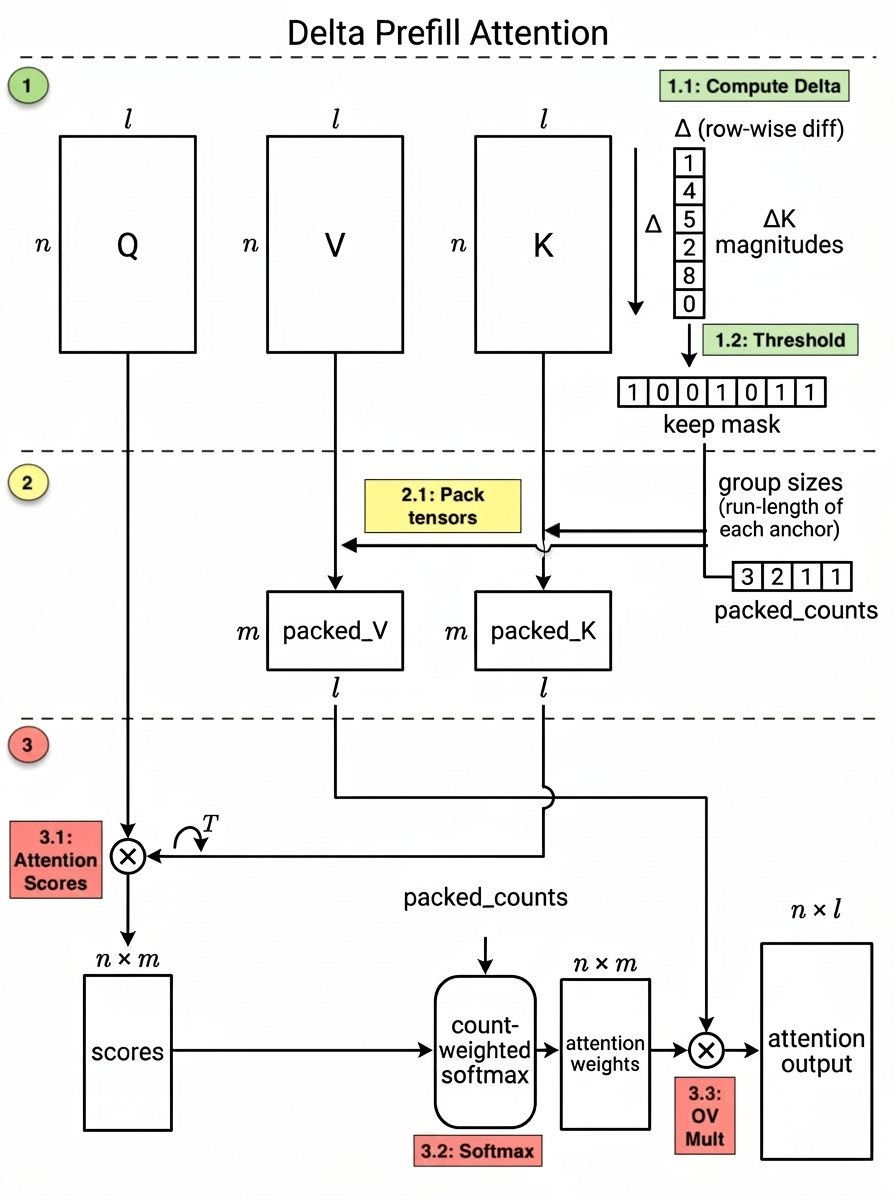
\includegraphics[width=0.65\textwidth]{../assets/delta_attention.jpeg}
    \caption{...}
    \label{fig:delta_attention}
\end{figure}

\subsection{(1) Pre-processing}

The pre-processing stage takes the key matrix $K$ as input and outputs a binary keep mask of length $n$. It analyzes $K$ row by row to decide which rows to keep and which to drop (steps 1.1 and 1.2 in Figure~\ref{fig:delta_attention}).

We initialize a keep mask of length $n$ to all ones, meaning all rows are initially kept. The anchor is set to the first row $K_0$. We then iterate over the remaining rows:

\begin{enumerate}
    \item Compute the Euclidean distance from row $K_i$ to the current anchor:
    \begin{equation}
        \delta_i = \| K_i - \text{anchor} \|_2
    \end{equation}
    \item If $\delta_i > \tau$ for some threshold $\tau$: the row is sufficiently different from the anchor, so we keep it and move the anchor to $K_i$.
    \item If $\delta_i \leq \tau$: the row is similar enough that the anchor can represent it, so we drop it by setting $\text{keepmask}[i] = 0$ and leave the anchor unchanged.
\end{enumerate}

The output keep mask has a 1 at each anchor position and a 0 at each dropped position.

\subsection{(2) Packing}

The packing stage takes the keep mask from stage (1) as input and outputs compressed key and value matrices $\hat{K}$ and $\hat{V}$, and a vector $\text{packed\_counts}$ (step 2.1 in Figure~\ref{fig:delta_attention}).

We drop all rows of $K$ and $V$ where the keep mask is 0, keeping only the anchor rows. The resulting $\hat{K}$ and $\hat{V}$ have shape $m \times l$, where $m < n$ is the number of anchors.

We also compute $\text{packed\_counts}$ of length $m$, where $\text{packed\_counts}[j]$ is the run length of anchor $j$, the number of rows it represents including itself.

\subsection{(3) Self-Attention}

The final stage takes the original query matrix $Q$ and the packed matrices $\hat{K}$, $\hat{V}$, and $\text{packed\_counts}$ from stage (2) as input, and outputs the attention output of shape $n \times l$. It follows the same steps as standard self-attention (Section~\ref{sec:self_attention}), with two differences: $Q$ is multiplied against the compressed $\hat{K}$ and $\hat{V}$ instead of the full matrices, and the softmax is weighted by $\text{packed\_counts}$.

\begin{enumerate}
    \item \textbf{Attention scores} (step 3.1): Multiply $Q$ by $\hat{K}^\top$ to get the score matrix:
    \begin{equation}
        S = \frac{Q\hat{K}^\top}{\sqrt{l}}
    \end{equation}
    $S$ has shape $n \times m$, where entry $(i, j)$ encodes how much token $i$ attends to anchor $j$.

    \item \textbf{Count-weighted softmax} (step 3.2): An anchor representing many tokens should have a proportionally larger effect than one representing a single token. To account for this, we scale each column of $S$ by the corresponding entry in $\text{packed\_counts}$ before applying the softmax:
    \begin{equation}
        \label{eq:count_weighted_softmax}
        W_{i,j} = \frac{\text{packed\_counts}[j] \cdot \exp(S_{i,j})}{\displaystyle\sum_{k=1}^{m} \text{packed\_counts}[k] \cdot \exp(S_{i,k})}
    \end{equation}
    For example, if token $i$ attends to anchor $j$ with score 5 and anchor $j$ represents 10 tokens, the score is updated to 50 before the softmax. This is equivalent to running standard self-attention where the anchor key vector is copied to all token positions it represents.

    \item \textbf{Attention output} (step 3.3): Multiply the attention weights by the packed value matrix:
    \begin{equation}
        \text{output} = W\hat{V}
    \end{equation}
    The compressed sequence dimension $m$ disappears after this multiplication, giving an output of shape $n \times l$ ,identical in shape to the output of standard self-attention.
\end{enumerate}

\subsection{Flash Attention Integration}

To test DeltaAttention on long context tasks we modified Flash Attention 2 to operate on the compressed $\hat{K}$ and $\hat{V}$ matrices. The kernel follows the same structure as FlashAttention 2 (Section~\ref{sec:flashattention_algorithm}): an outer loop over query blocks, with each kernel program handling one query block independently. The inner loop is modified to operate in two phases.

Alongside $\hat{K}$, $\hat{V}$, and $\text{packed\_counts}$, we store a $\texttt{packed\_timestamps}$ vector of length $m$. Entry $j$ holds the index in the original sequence of the last token that anchor $j$ represents. For example, if anchor $j$ represents tokens 5, 6, and 7 from the original sequence, then $\texttt{packed\_timestamps}[j] = 7$. This vector can be computed as a cumulative sum of $\text{packed\_counts}$, minus one. It lets the kernel track how far into the original sequence each anchor's coverage extends.

\textbf{Phase 1: Compressed history.} The first phase iterates over blocks of $\hat{K}$ and $\hat{V}$ instead of blocks of $K$. For each packed block, the kernel reads the $\texttt{packed\_timestamps}$ of the anchors in that block and takes their maximum. This is the reach of the block: the furthest position in the original sequence that any anchor in the block represents.

We define the \textbf{critical diagonal} of a query block as the span of positions the block itself covers, $[\text{query\_block\_start},\, \text{query\_block\_end}]$. Any anchor whose reach falls within this span represents tokens that overlap with the current query block and must be processed exactly. This follows the local attention window principle described in Section~\ref{sec:local_attention_window}: tokens attend most strongly to their immediate neighbors, so those neighbors must be kept exact.

If the reach falls before the critical diagonal (reach $<$ query\_block\_start), the block is safe to process in compressed form. The kernel computes the attention scores against the packed key vectors and applies count-weighted softmax exactly as in Equation~\ref{eq:count_weighted_softmax}, updating the online softmax running state ($m_i$, $l_i$, $\text{acc}$) as in standard FlashAttention.

If the reach falls inside or past the critical diagonal, the first phase stops. Those anchors cover tokens that belong to the current query block, so they need to be processed exactly.

\textbf{Phase 2: Critical diagonal.} The second phase switches to the original uncompressed $K$ and $V$. Starting from just after the last safe anchor's reach and going up to the end of the current query block, it runs standard FlashAttention over the exact token vectors.





